\documentclass[../Cours.tex]{subfiles}

\begin{document}
\clearpage
\thispagestyle{empty}

\setcounter{DS}{2}

\color{black}
\nomPrenom{}
\titreDS

\begin{questions}
    \EXERCICETITRE{4}{Volume d'un tore}
    Un tore est un solide en forme d'anneau. Pour calculer le volume d'un tore, on utilise la formule suivante : $V_{\mbox{tore}} = 2\pi^2r^2R$ avec $r$ le petit rayon et $R$ le grand rayon.

    \question Calculer le volume d'un tore de petit rayon \qty{3}{\centi\metre} et de grand rayon \qty{5}{\centi\metre}.
    \question Calculer le volume d'un tore de petit rayon \qty{4}{\centi\metre} et de grand rayon \qty{4}{\centi\metre}.

    \EXERCICETITRE{4}{Suite de figures}
    \begin{center}
    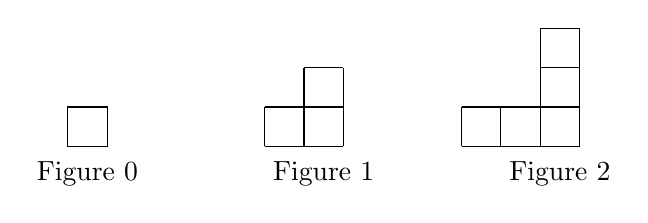
\begin{tikzpicture}[scale=0.5]
        \draw (0,0) rectangle (1,1);
        \node at (0.5,-0.7) {Figure 0};
        \draw (5,0) grid (7,1);
        \draw (6,0) grid (7,2);
        \node at (6.5,-0.7) {Figure 1};
        \draw (10,0) grid (13,1);
        \draw (12,0) grid (13,3);
        \node at (12.5,-0.7) {Figure 2};
    \end{tikzpicture}
    \end{center}

    En poursuivant cette suite de figures, combien y aura-t-il de carrés...
    \question pour la figure 3 ?
    \question pour la figure 10 ?
    \question pour la figure 100 ?
    \question pour la figure $n$ ?

    \EXERCICETITRE{4}{Ballon de football}
    Un ballon de football a pour rayon \qty{11.98}{\centi\metre}. 

    \question Quel est le volume du ballon ? (rappel : $V_{\mbox{boule}} = \frac{4}{3} \pi r^3$)
    
    \question Pour s'assurer du bon déroulement du match, on a besoin d'au moins 5 ballons. Quel sera alors le volume total des ballons de football ?

    \EXERCICETITRE{4}{THALÈS}

    \begin{center}
    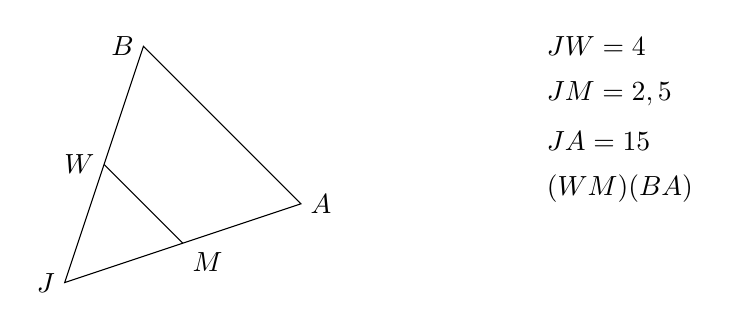
\begin{tikzpicture}
        \draw (0,0) node[left]{$J$} -- (1,3) node[left]{$B$} -- (3,1) node[right]{$A$} -- cycle;
        \draw (0.5,1.5) node[left]{$W$} -- (1.5,0.5) node[below right]{$M$};
        \node[anchor=west] at (6,3) {$JW = 4$};
        \node[anchor=west] at (6,2.4) {$JM = 2,5$};
        \node[anchor=west] at (6,1.8) {$JA = 15$};
        \node[anchor=west] at (6,1.2) {$(WM) \paral (BA)$};
    \end{tikzpicture}
    \end{center}

    \question Déterminer $JB$

    \EXERCICETITRE{4}{THALÈS ET PYTHAGORE}

    $ABR$ est un triangle rectangle $B$, tel que $AB = 13$ et $BR = 18$. \\
    Placer $I$ sur $[AB]$ tel que $AI=4$. \\
    On trace une droite $(d)$ perpendiculaire à $(AB)$ passant par $I$, coupant $(AR)$ en $J$.

    \question Calculer $AR$
    \question Calculer $IJ$

    
\end{questions}
\end{document}